\documentclass[11pt]{article}

\usepackage[margin=1in]{geometry}
\usepackage{graphicx}
\usepackage{booktabs}
\usepackage{amsmath}
\usepackage{amssymb}
\usepackage{hyperref}
\usepackage{enumitem}
\usepackage{xcolor}

\title{The Visual Folio Machine: Image-Native Reading, Memory, and Writing}
\author{Imagized Language Model Project}
\date{August 2026}

\begin{document}
\maketitle

\begin{abstract}
Most language models represent language through symbolic tokens and treat visible writing as an auxiliary modality. We investigate a stricter object: an independent model that receives writing images, forms continuous visual states, and returns image-valued answers. Three implementations falsify convenient shortcuts. Whole-page rectified flow learns page texture but not legible language; a pooled visual embedding does not retrieve semantic paraphrases reliably; and an 8-pixel causal writing stream reaches teacher-forced ink F1 0.639 while autonomous output collapses to repeated grey marks. These results motivate the Visual Folio Machine (VFM): an ordered axial retina distilled offline into a centered continuous semantic field, an image-keyed and image-valued associative folio, an evidence gate that copies attested historical forms, and a future whole-field masked writer for novel connective prose. The deployed reader contains no vocabulary, text IDs, OCR transcript, or external language-model call. This paper defines the model boundary, equations, one-RTX-4090 implementation, falsifiable benchmark, and limits of the present proof.
\end{abstract}

\begin{figure}[t]
  \centering
  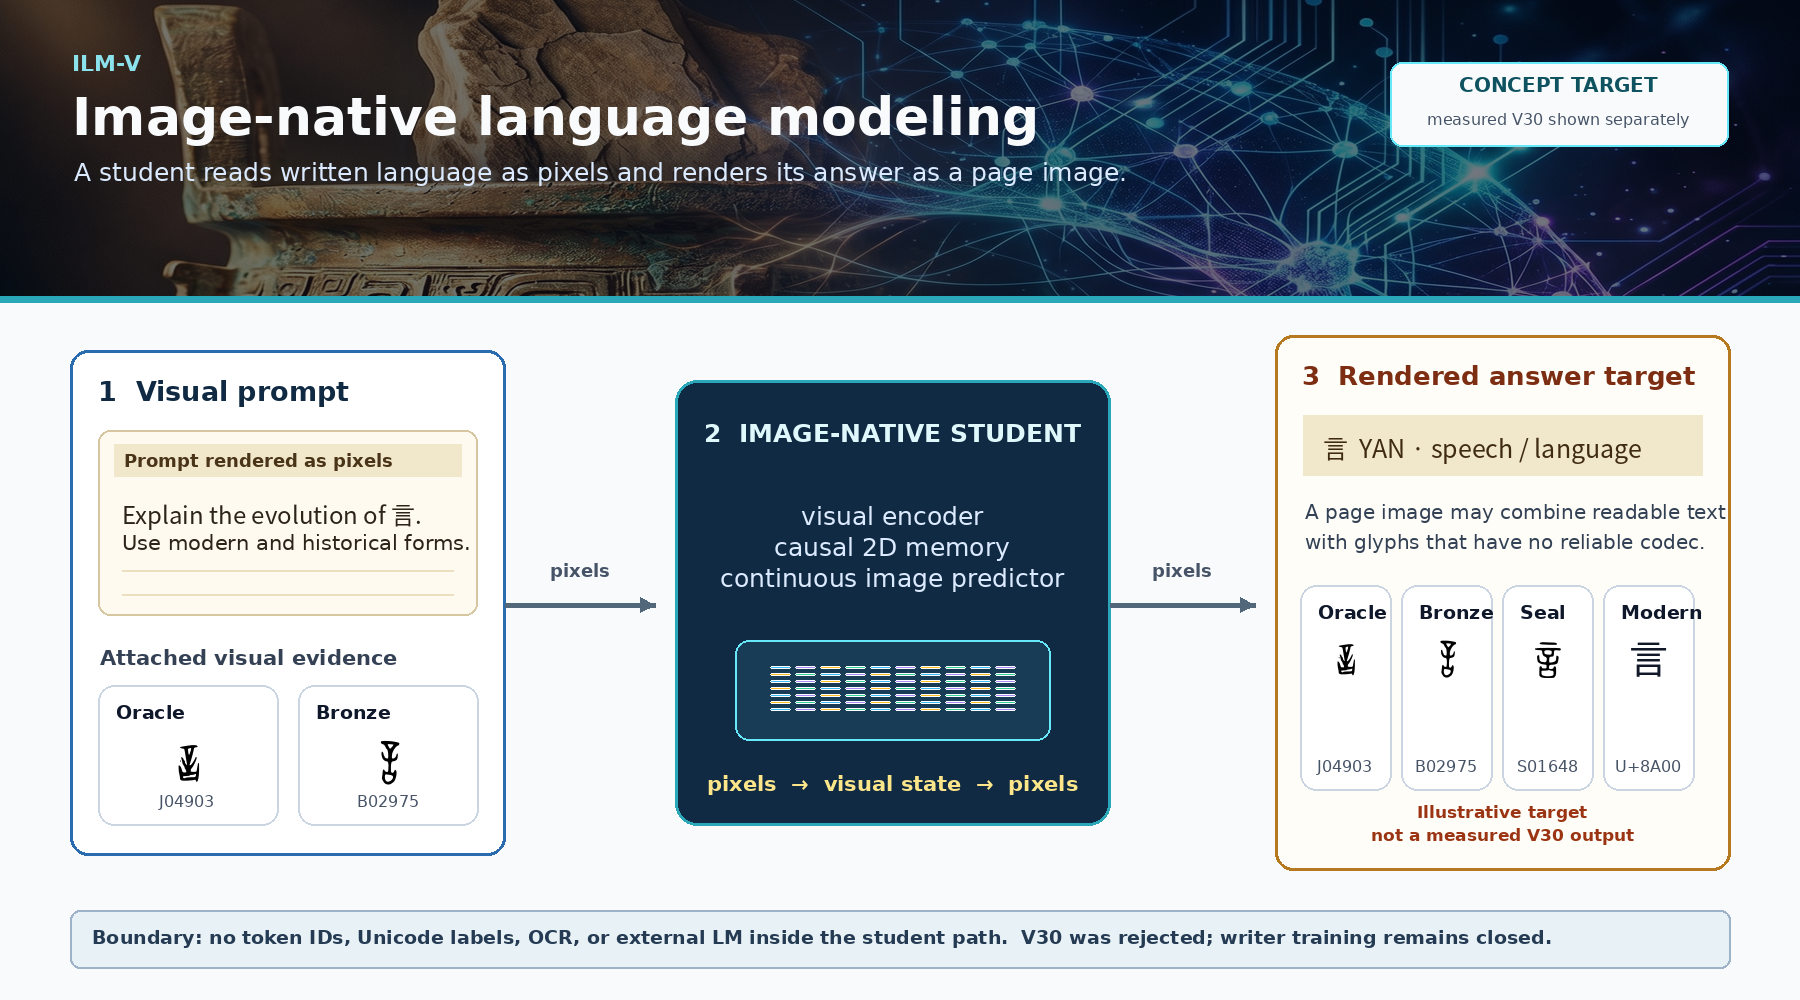
\includegraphics[width=\linewidth]{figures/ilm_v_yan_readme_hero.png}
  \caption{Image-native language modeling concept figure generated with an AgInTi background and overlaid with real local ziyuan glyph exemplars for \texttt{YAN} (U+8A00). The answer is a rendered image containing both modern explanation and historical forms.}
  \label{fig:yanhero}
\end{figure}

\section{Motivation}

Human readers do not see byte-pair tokens. They see pages, lines, strokes, spacing, damage, font variation, and script-specific visual forms. Current language models are extremely capable, but their central representation is normally a sequence of text tokens. Multimodal models accept images, and modern APIs also expose image-generation endpoints. For example, OpenAI documents APIs for processing images as input and generating images as output, and Google's Gemini API documentation describes image generation from text and image prompts~\cite{openaiimages,openaiimagegen,geminiimage}. These systems are important baselines, but they do not by themselves define a language model whose primary language substrate is the visible page.

The Imagized Language Model (ILM) goal is different:
\[
\text{image input} \rightarrow \text{visual language state} \rightarrow \text{image output}.
\]
The output should itself be a readable answer image. For a query such as ``explain the evolution of character yan'', the system should produce a page containing modern explanatory writing, classical-style Chinese, and oracle, bronze, seal, and modern forms. Typed text can still be accepted by a user interface, but it is rasterized into an image prompt before entering the core model. Conversely, the model's answer is a page image first; OCR or transcription is an optional downstream extraction step.

\section{Prior Art and Gap}

OCR-free document models such as Donut and screenshot parsing models such as Pix2Struct show that document images can be understood without an explicit OCR pipeline. PIXEL reconstructs masked rendered-text patches and demonstrates cross-script visual transfer~\cite{pixel}; PIXAR is a genuinely generative pixel-space autoregressive language model and identifies noisy maximum-likelihood text images as a central difficulty~\cite{pixar}; PixelGPT studies autoregressive visual and textual pretraining~\cite{pixelgpt}. These are the closest model-level precedents. Token-free language models such as CANINE, ByT5, and MEGABYTE remove subwords but retain symbolic bytes or characters. Discrete diffusion language models show that generation need not be left-to-right, but usually retain a linguistic vocabulary.

The remaining gap is not simply ``pixels instead of tokens.'' It is a system that (i) preserves ordered visual evidence, (ii) acquires semantic neighborhoods without retaining a text teacher, (iii) outputs exact image values when the answer already exists, and (iv) never presents a synthesized historical-looking mark as attested evidence. VFM addresses the first three in runnable code and makes the fourth an explicit provenance contract. Unrestricted novel image writing remains an open stage rather than an implied result.

\section{Architecture}

\begin{figure}[t]
  \centering
  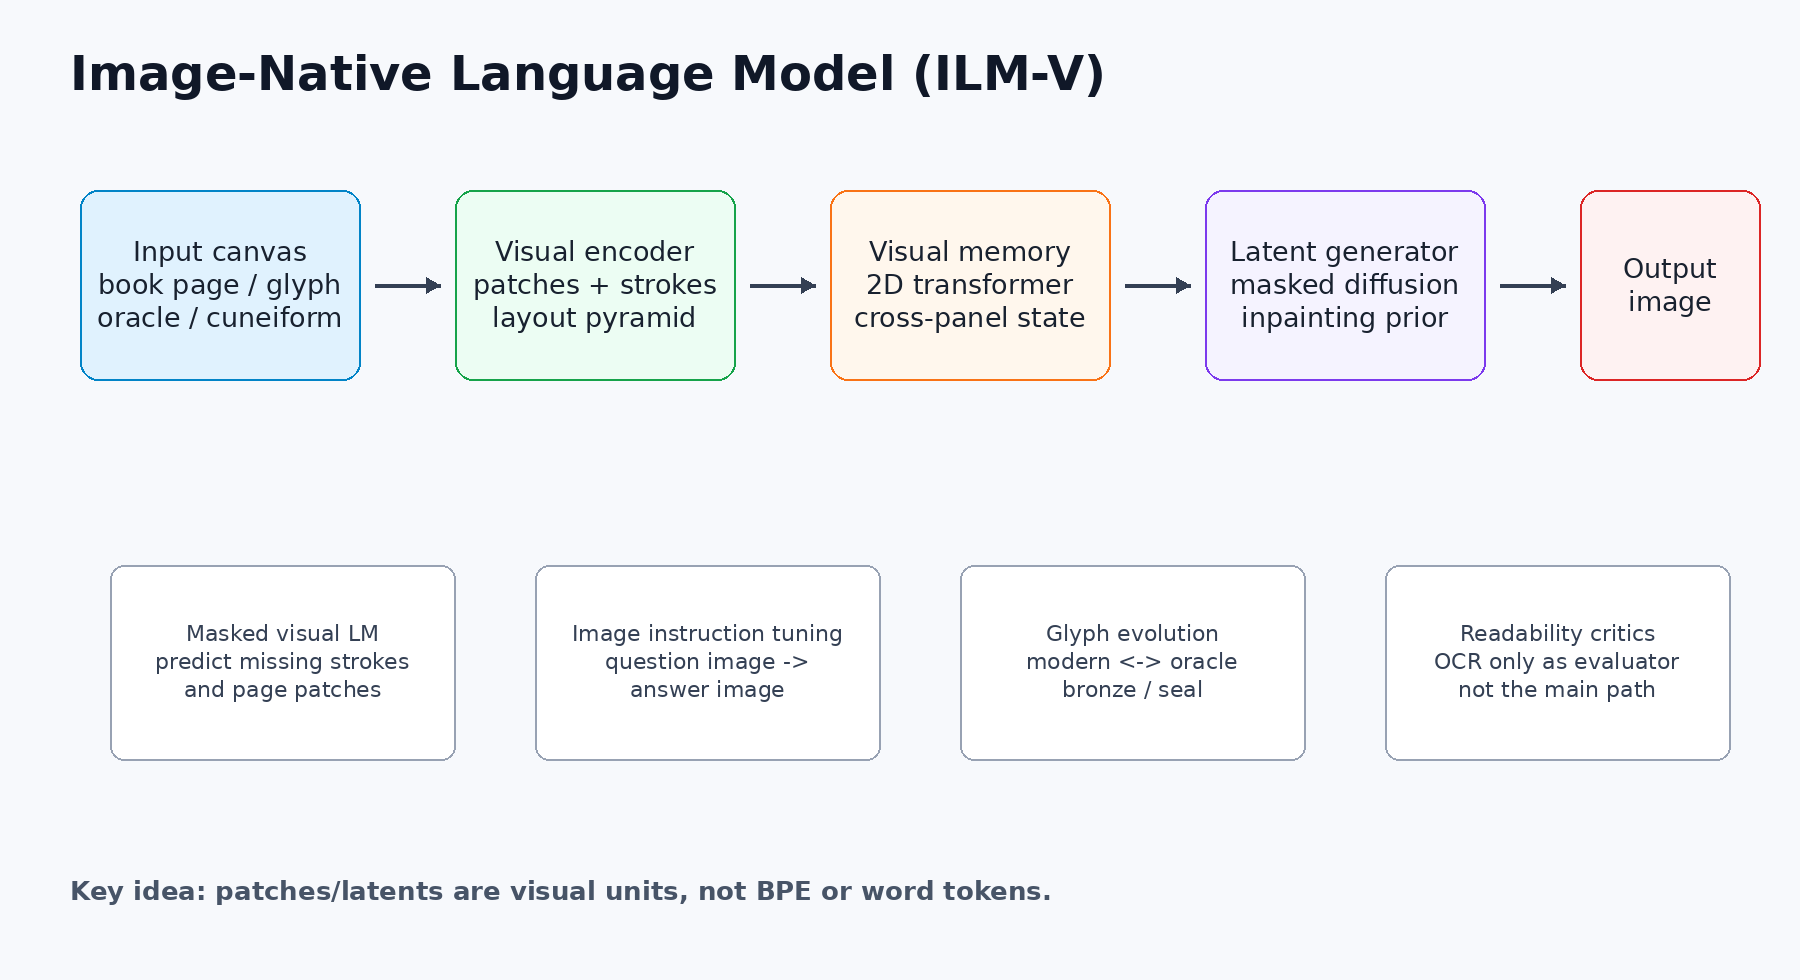
\includegraphics[width=\linewidth]{figures/architecture_overview.png}
  \caption{Conceptual image-native architecture. The implemented VFM specializes this design into an ordered axial retina, a continuous semantic field, an image-valued folio, and a provenance gate. Whole-field masked writing is the next stage.}
  \label{fig:architecture}
\end{figure}

Figure~\ref{fig:architecture} gives the visual contract. The implemented system has four separable components:
\begin{enumerate}[leftmargin=*]
  \item \textbf{Ordered folio retina.} A stroke-preserving convolutional stem maps a grayscale writing image to a stride-16 field. Alternating axial attention reads along writing lines and exchanges evidence between lines without assigning patches lexical identities.
  \item \textbf{Centered semantic field.} A local multilingual embedding model supplies continuous fields during offline training only. Corpus anisotropy is removed before distillation; the deployed student contains neither teacher weights nor calls.
  \item \textbf{Image-valued folio.} Multiple student-derived visual keys address exact answer-page images. Runtime manifests contain paths and provenance but deliberately omit prompt and answer strings.
  \item \textbf{Evidence and writing gates.} Attested historical glyphs are copied from source pixels. Novel prose is reserved for a masked whole-answer canvas refiner, so a weak generator cannot silently replace evidence.
\end{enumerate}

For image $X\in[0,1]^{H\times W}$, the retina produces $F\in\mathbb{R}^{H/16\times W/16\times d}$. One axial block computes
\[
F'_{r,:,:}=F_{r,:,:}+\operatorname{Attn}_{x}(F_{r,:,:}),\quad
F''_{:,c,:}=F'_{:,c,:}+\operatorname{Attn}_{y}(F'_{:,c,:}).
\]
Ink-aware pooling and projection produce $s_\theta(X)\in\mathbb{S}^{D-1}$. There is no embedding lookup or language-classification head.

The raw teacher field is anisotropic. In the measured 10,000-document Chinese cache, unrelated pairs average cosine 0.360 and the mean-vector norm is 0.597. Therefore
\[
\mu=\frac{1}{N}\sum_i t_i,\qquad r_i=\frac{t_i-\mu}{\lVert t_i-\mu\rVert_2}
\]
is the target. Centering reduces mean unrelated cosine to approximately zero. Two visual augmentations $A_1,A_2$ of one document are trained with
\[
\mathcal{L}_{\mathrm{read}}=
\mathcal{L}_{\mathrm{cos}}(s(A_1X),r)+
\lambda_v\mathcal{L}_{\mathrm{cos}}(s(A_1X),s(A_2X))+
\lambda_r\lVert SS^\top-RR^\top\rVert_1+
\lambda_c\mathcal{L}_{\mathrm{NCE}}(S,R).
\]
At inference, $i^*=\arg\max_i\max_v s_\theta(X)^\top k_{iv}$, and the value is a sequence of image pages. The internal units remain continuous spatial observations, not BPE, wordpiece, Unicode, or renamed discrete visual tokens.

\section{Data}

The project already has a strong historical Chinese glyph source outside the tracked repo. A local snapshot at \texttt{/home/lachlan/ProjectsLFS/incoder/data/historic} contains:
\begin{center}
\begin{tabular}{lr}
\toprule
Item & Count \\
\midrule
Characters & 9,055 \\
Glyph records & 84,642 \\
Oracle & 32,216 \\
Bronze & 23,500 \\
Liushutong & 21,923 \\
Seal & 6,996 \\
\bottomrule
\end{tabular}
\end{center}

This supports evidence-bearing historical answer pages. The first semantic run additionally uses 5,000 CC-BY-NC-4.0 Chinese Alpaca instruction pairs, rendered into 10,000 prompt/answer folios. BGE-M3 fields are cached only for offline distillation. Public-domain scans remain a planned robustness corpus; source license, hash, and transform must be recorded before use.

\section{Training Objectives}

The current VFM curriculum separates objectives that previous runs incorrectly conflated:
\begin{enumerate}[leftmargin=*]
  \item \textbf{Visual reading:} align independently rendered folios to centered continuous teacher fields and preserve pairwise semantic geometry.
  \item \textbf{Visual addressing:} evaluate full-memory top-(k) retrieval under unseen typography before adding generation.
  \item \textbf{Paraphrase transfer:} use Qwen offline to rewrite held-out questions, reject meaning drift with an independent embedding threshold, rasterize the accepted rewrite, and test the independent student only.
  \item \textbf{Evidence output:} retrieve and copy exact historical glyph panels with source metadata.
  \item \textbf{Whole-field writing:} corrupt complete answer canvases and learn iterative masked revision conditioned on prompt and retrieved evidence. This stage is not credited until autonomous pages are legible.
\end{enumerate}

\section{Image-First Training and Inference}

\begin{figure}[t]
  \centering
  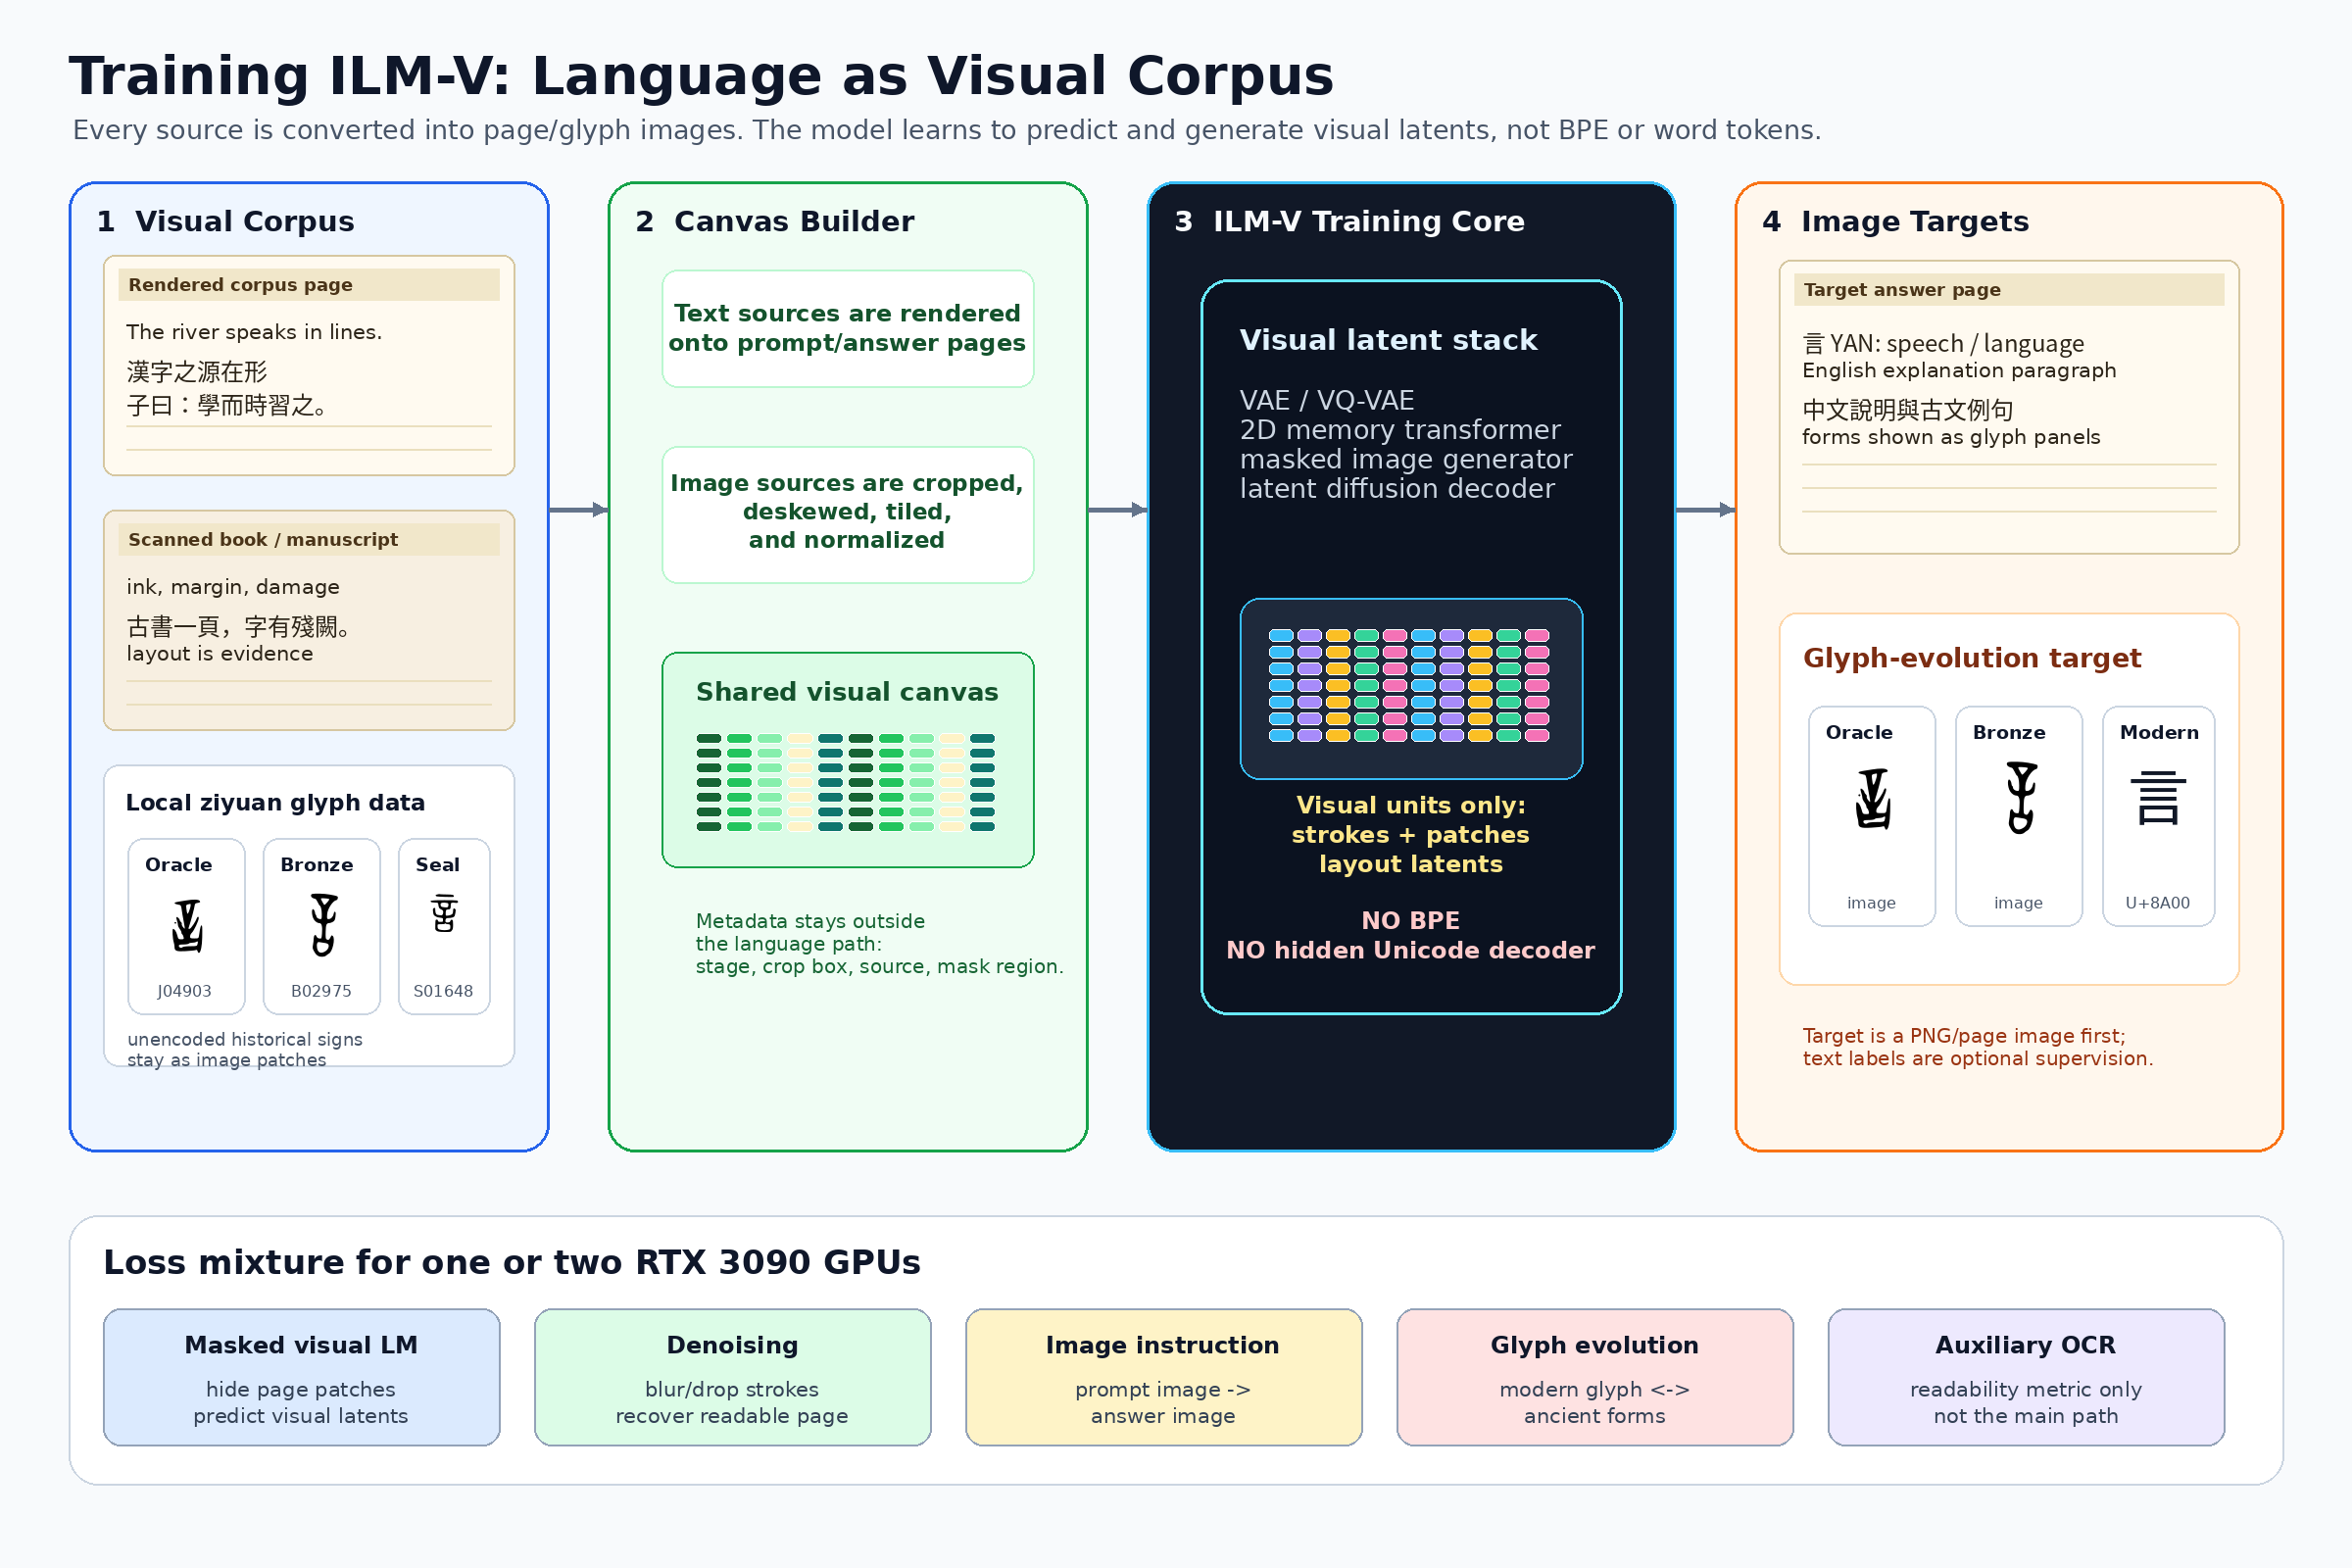
\includegraphics[width=\linewidth]{figures/visual_language_training_pipeline.png}
  \caption{Training pipeline for ILM-V. Rendered text corpora, scanned pages, historical glyph files, and unencoded marks are all converted into visual canvases. The training target is visual latent prediction and image generation, not BPE-token prediction.}
  \label{fig:visualtraining}
\end{figure}

Figure~\ref{fig:visualtraining} makes the training contract explicit. Typed corpora are rendered into page images; scanned books and manuscripts are cropped and tiled; historical glyph files become glyph tiles; and marks that are missing from font tables remain valid image patches. Metadata such as crop boxes and stage labels may remain in manifests, but the model path should learn from visual latents. OCR is useful as a readability critic, not as the hidden language channel.

\begin{figure}[t]
  \centering
  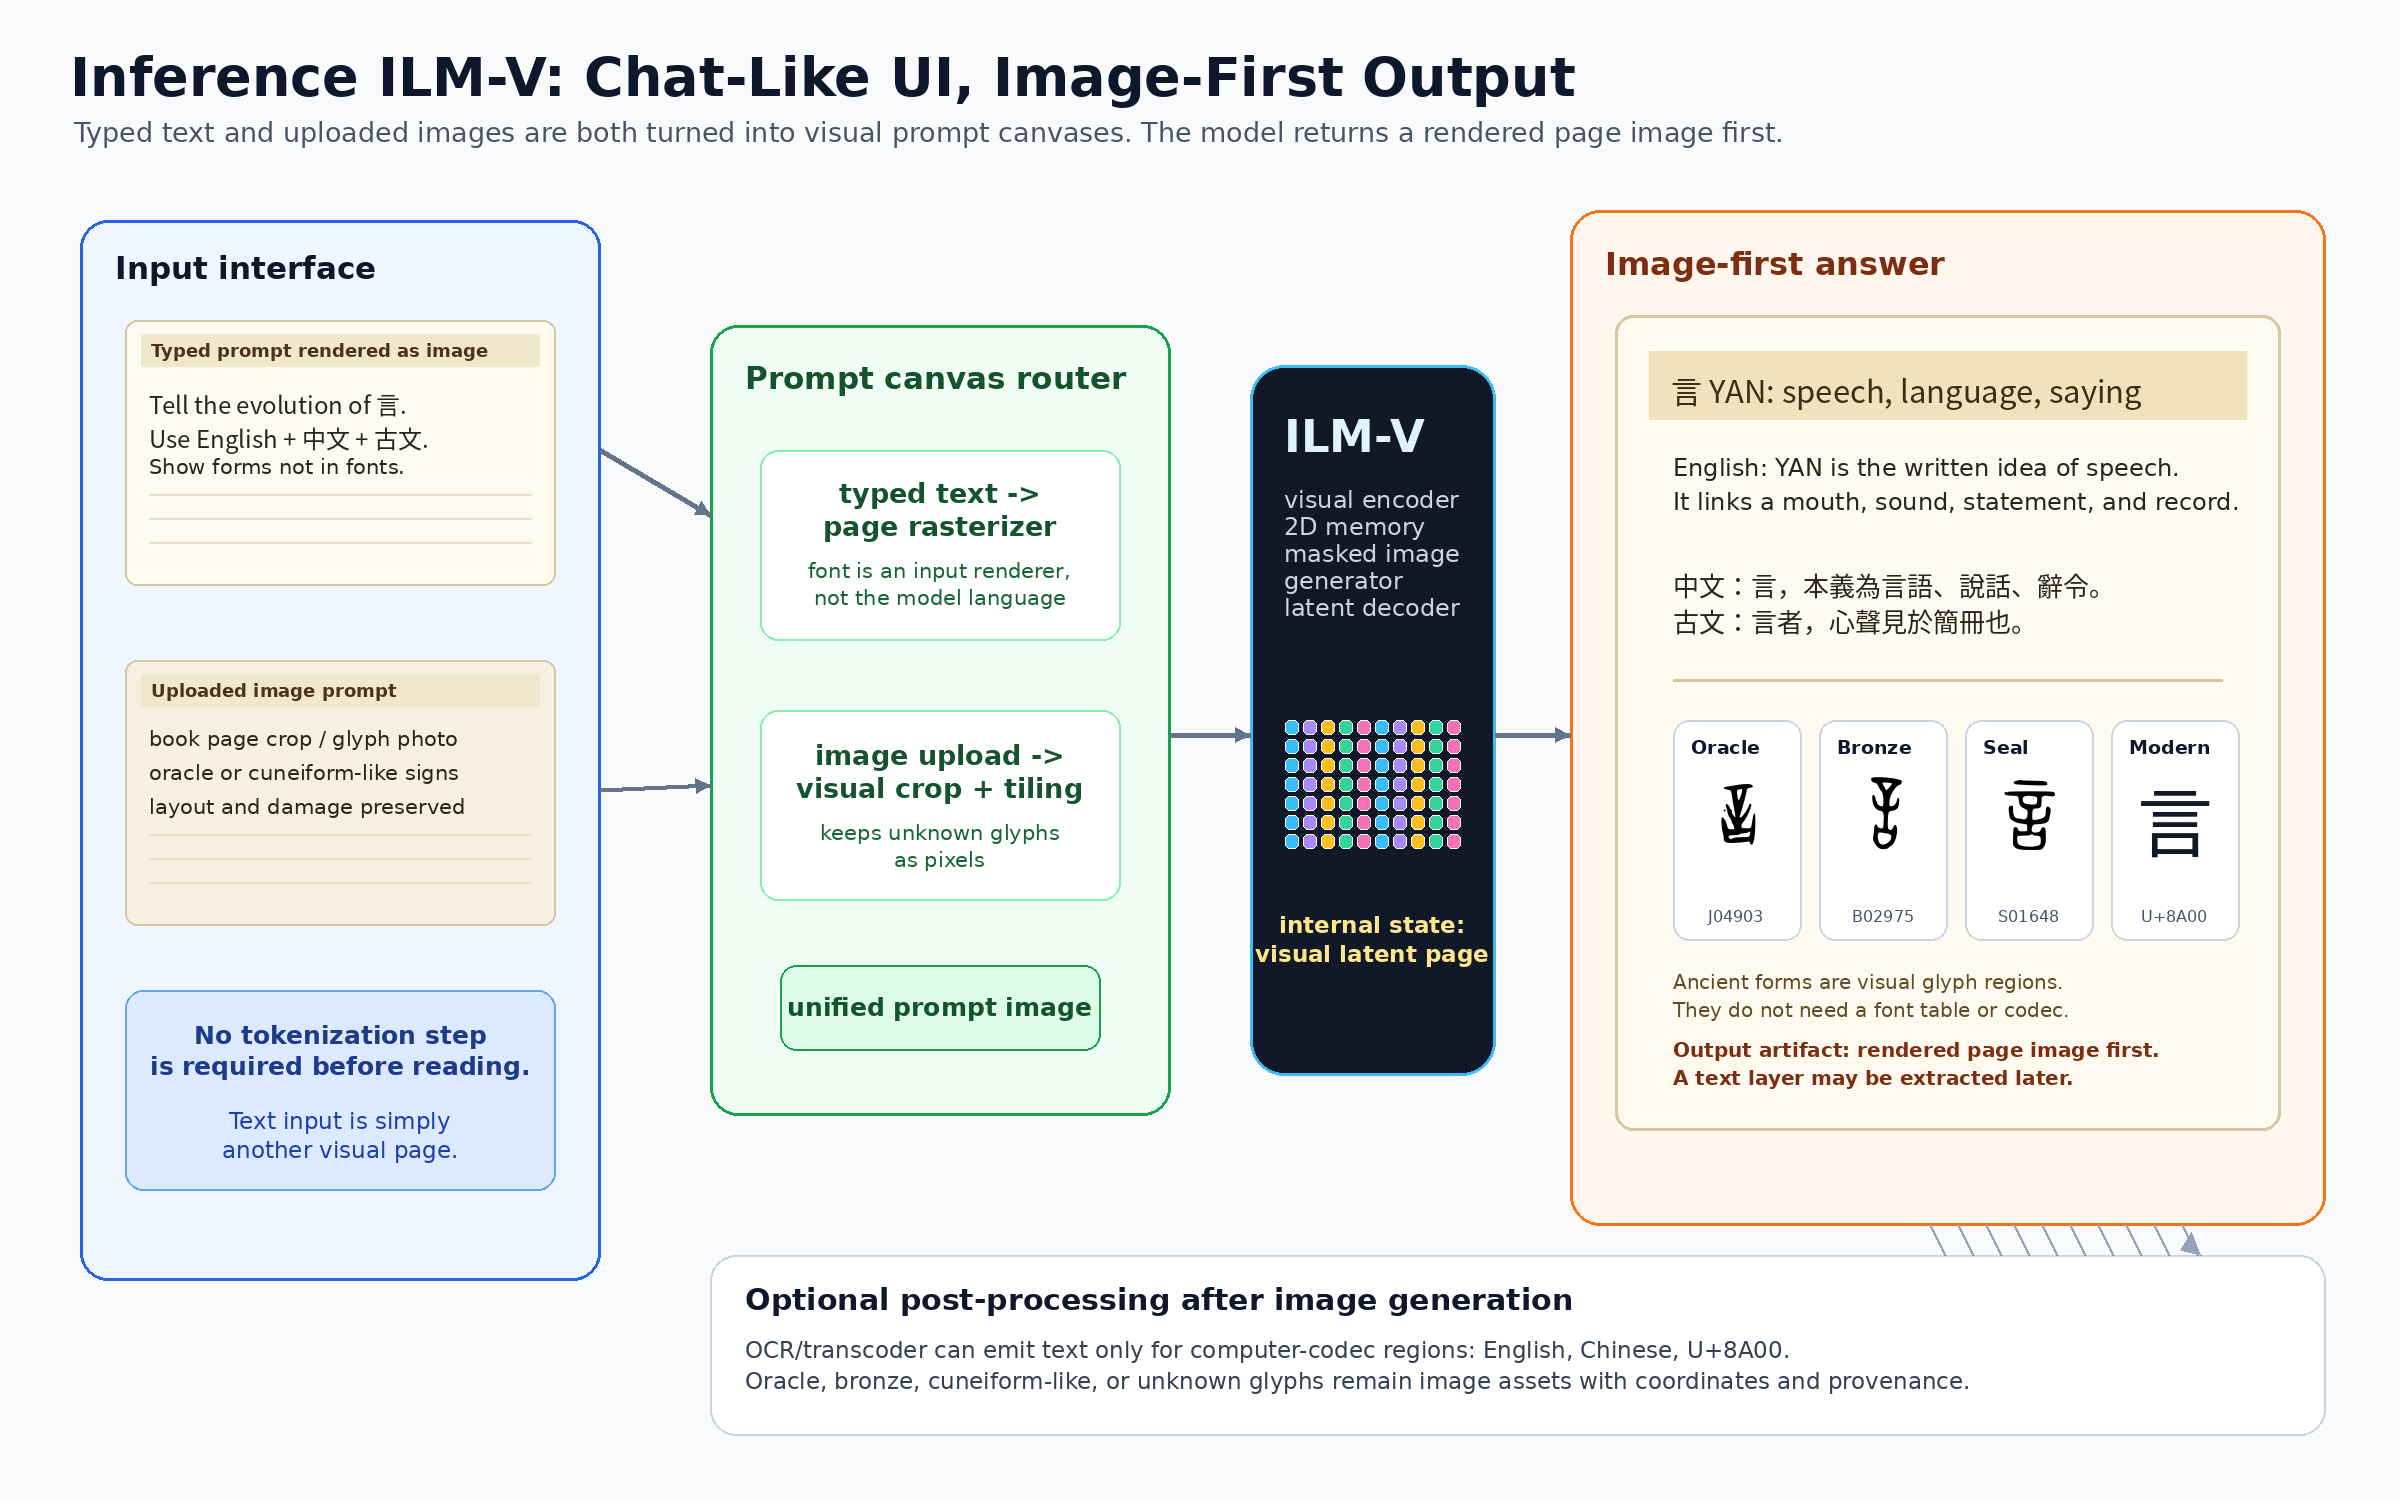
\includegraphics[width=\linewidth]{figures/visual_language_inference_pipeline.png}
  \caption{Inference pipeline for ILM-V. A chat-like interface may accept typed text or uploaded images, but typed text is first rasterized into a prompt image. The primary output is a rendered page image. OCR or transcoding is optional and only applies to output regions that exist in computer codecs.}
  \label{fig:visualinference}
\end{figure}

Figure~\ref{fig:visualinference} shows the user-facing path. A typed prompt is converted into a visual prompt canvas, and an uploaded image is normalized into the same visual space. The model returns a page-like image containing modern language and historical glyph regions. A later OCR/transcoder can attach a searchable text layer for English, Chinese, or Unicode-representable spans; ancient or unencoded glyphs remain image regions with coordinates and provenance.

The formal contract is:
\[
\begin{aligned}
r_\alpha(\text{text prompt}) &\rightarrow x_{\mathrm{prompt}},\\
g_\beta(\text{uploaded page or glyph}) &\rightarrow x_{\mathrm{prompt}},\\
f_\theta(x_{\mathrm{prompt}}, x_{\mathrm{context}}) &\rightarrow y_{\mathrm{page}},\\
o_\psi(y_{\mathrm{page}}) &\rightarrow \text{optional text layer} + \text{glyph-region metadata}.
\end{aligned}
\]
Here \(r_\alpha\) is only a UI rasterizer, not the language model itself. The core model \(f_\theta\) maps visual inputs to a rendered page image \(y_{\mathrm{page}}\). The optional reader \(o_\psi\) may recover Unicode text where possible, but unencoded historical forms remain valid image regions.

A useful answer canvas should resemble a page excerpt from a book or corpus:
\begin{itemize}[leftmargin=*]
  \item a title region rendered as text image,
  \item one or more modern-language paragraphs, for example English and Chinese,
  \item a classical-style line or quotation when appropriate,
  \item glyph panels for forms that may not exist in computer fonts,
  \item a provenance strip with source IDs or nearest retrieved exemplars.
\end{itemize}

This schema is intentionally different from ``text answer plus illustrations''. The generated page image is the primary output object, and the text layer is secondary.

\section{3090-Friendly Curriculum}

\begin{figure}[t]
  \centering
  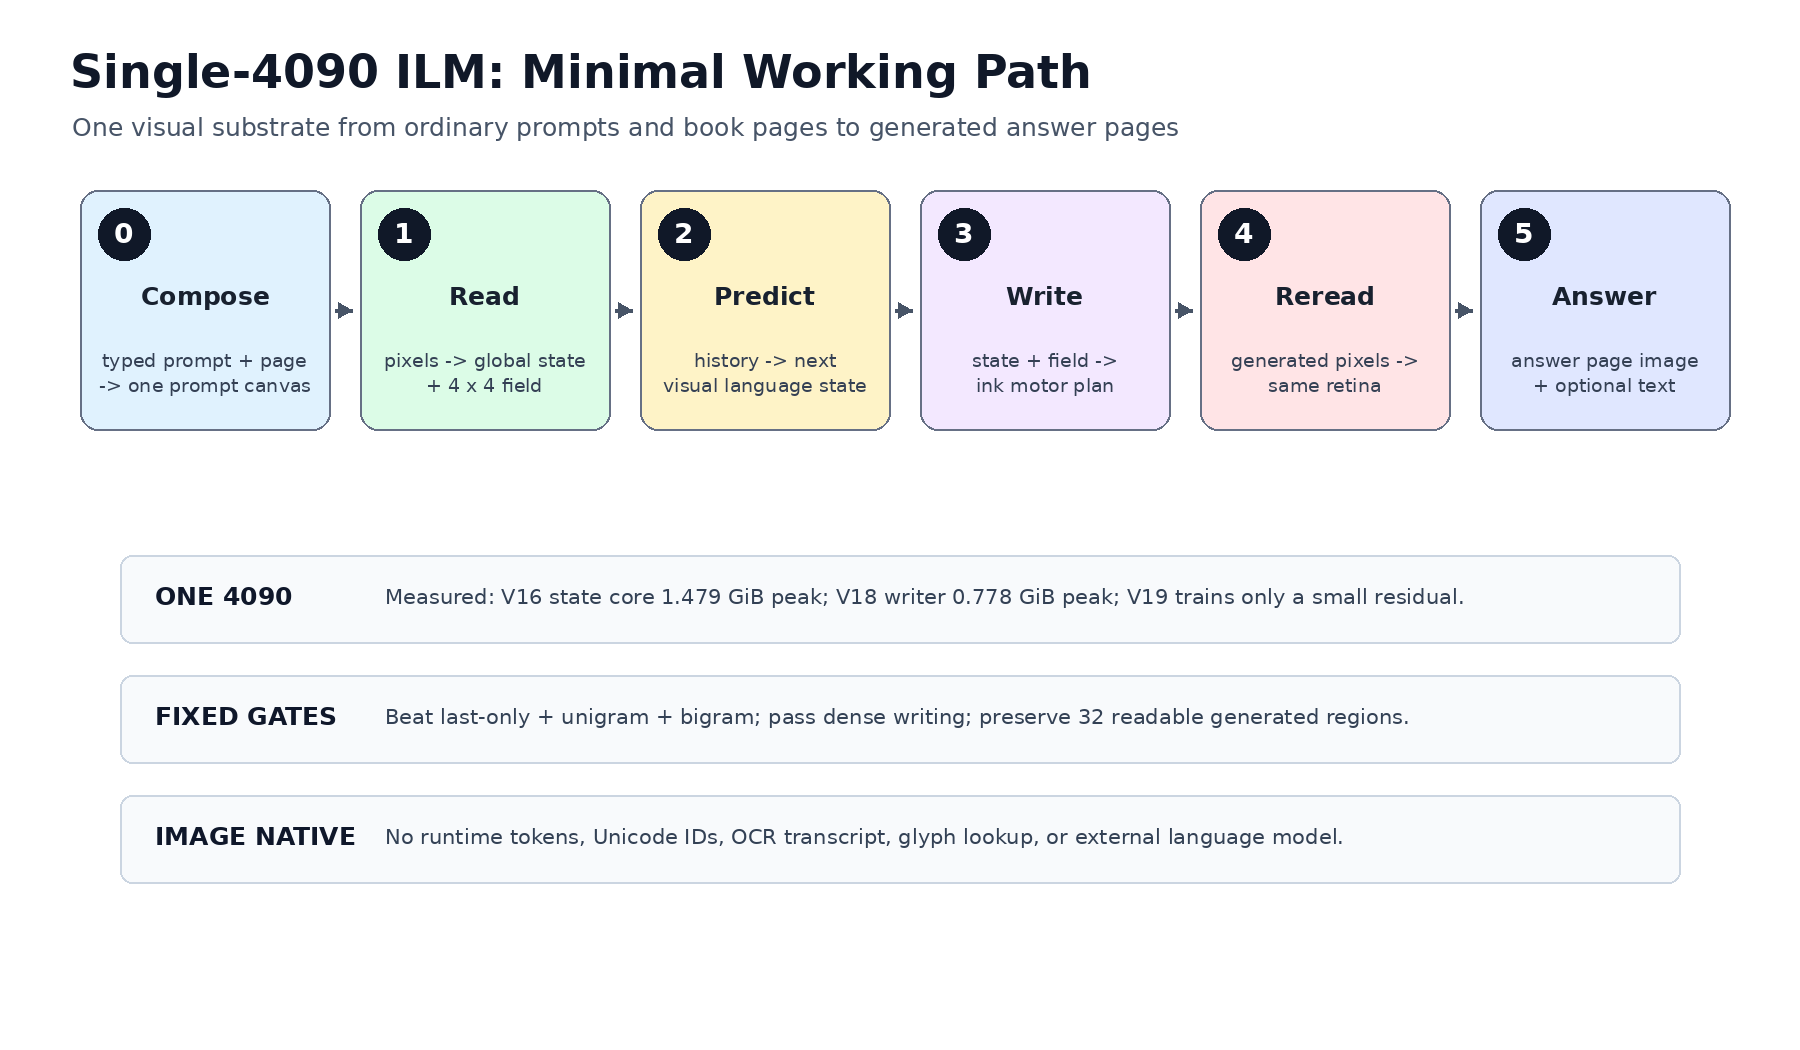
\includegraphics[width=\linewidth]{figures/training_curriculum.png}
  \caption{A staged curriculum that fits one or two RTX 3090 GPUs by starting with glyph tiles and latent generation before scaling to page-level image language modeling.}
  \label{fig:curriculum}
\end{figure}

Figure~\ref{fig:curriculum} illustrates the original schedule. Measurements support a revised, lower-risk order:
\begin{enumerate}[leftmargin=*]
  \item Train the 10.9M-parameter ordered retina on rendered instruction folios.
  \item Prove full-memory semantic retrieval, held-out typography, and held-out paraphrases.
  \item Insert evidence-bearing historical pages without retraining and verify multilingual queries.
  \item Train a compact whole-field writer over retrieved answer layouts rather than pages sampled from pure noise.
  \item Add public-domain book crops and manuscript damage to the retina curriculum.
  \item Scale width, memory, and answer composition only after bounded comparisons justify it.
\end{enumerate}

The retina is deliberately small enough for one 24GB RTX 4090. The first 10,000-field teacher cache took 55 seconds locally. All speed, VRAM, and accuracy numbers must be measured again on the finalized checkpoint; ``more efficient than an LLM'' is a hypothesis until a named benchmark supports it.

\section{Target Demonstration}

\begin{figure}[t]
  \centering
  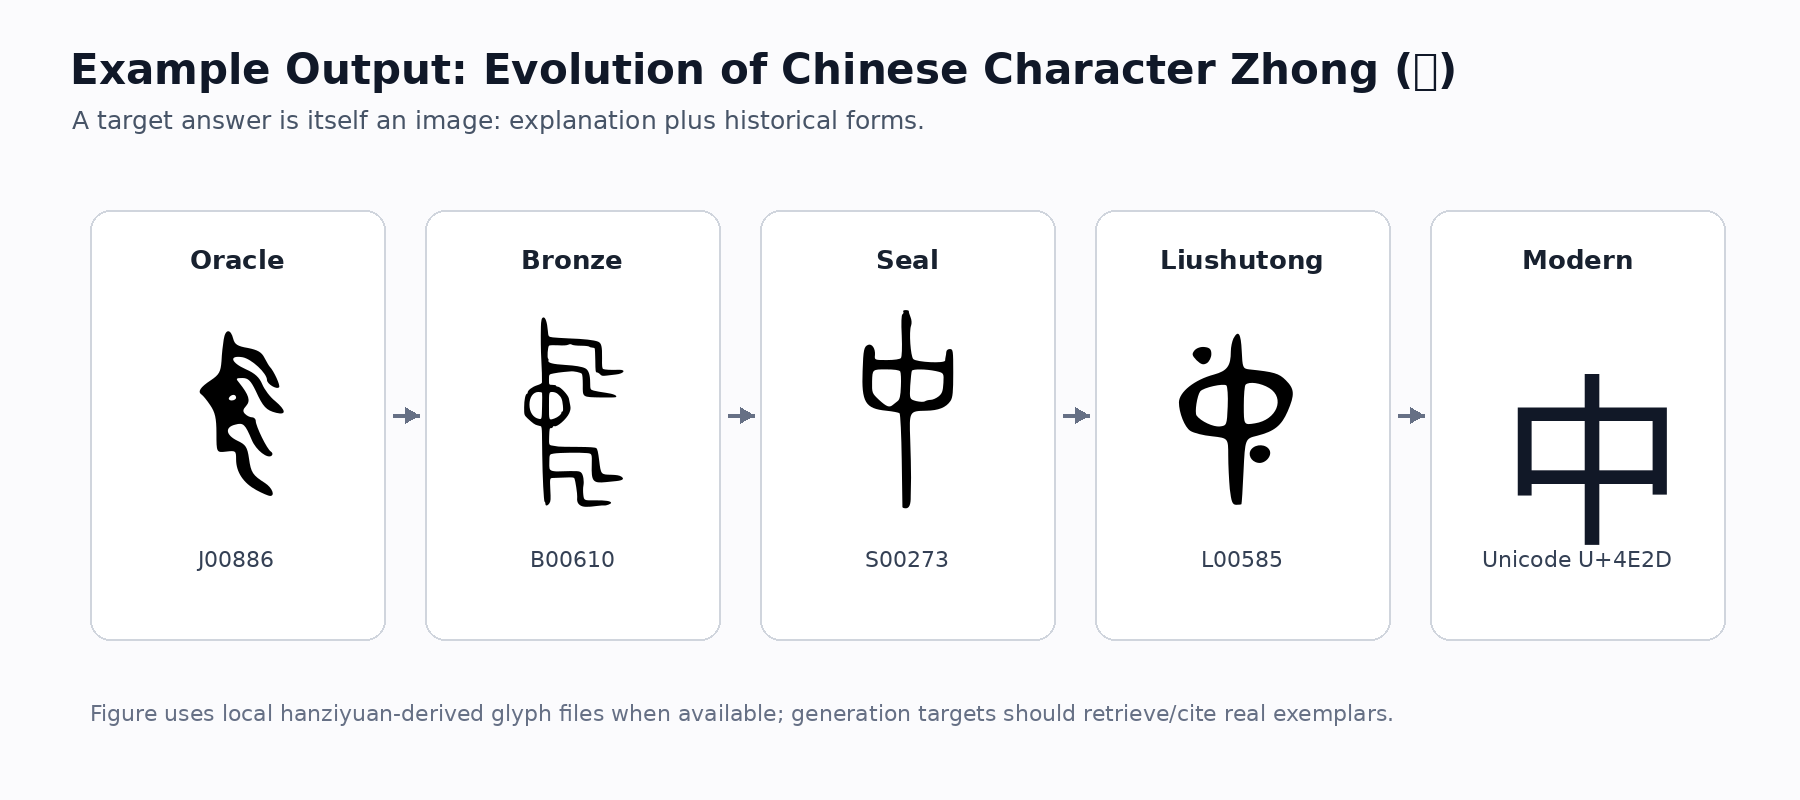
\includegraphics[width=\linewidth]{figures/zhong_evolution_example.png}
  \caption{Target output style for a glyph-evolution question. The answer is not merely text: it is a readable image with historical visual forms. The example uses local hanziyuan-derived glyph files when available.}
  \label{fig:zhong}
\end{figure}

The first demo should answer a rendered visual prompt such as: ``Explain the evolution of the Chinese character yan.'' The target answer image should contain:
\begin{itemize}[leftmargin=*]
  \item a title and concise modern explanation,
  \item English and Chinese paragraphs rendered as page text,
  \item a classical-style line such as ``yan is the visible trace of speech'',
  \item a historical timeline with real oracle, bronze, seal, and modern glyph exemplars,
  \item stage labels and citations as rendered image text.
\end{itemize}

The existing Zhong figure in Figure~\ref{fig:zhong} is a compact stage-timeline example; the Yan figures in Figures~\ref{fig:yanhero} and~\ref{fig:visualinference} show the fuller answer-page style. Together they test whether the model can combine language understanding, visual page composition, and historical script generation.

\section{AgInTi Artifact Loop}

\begin{figure}[t]
  \centering
  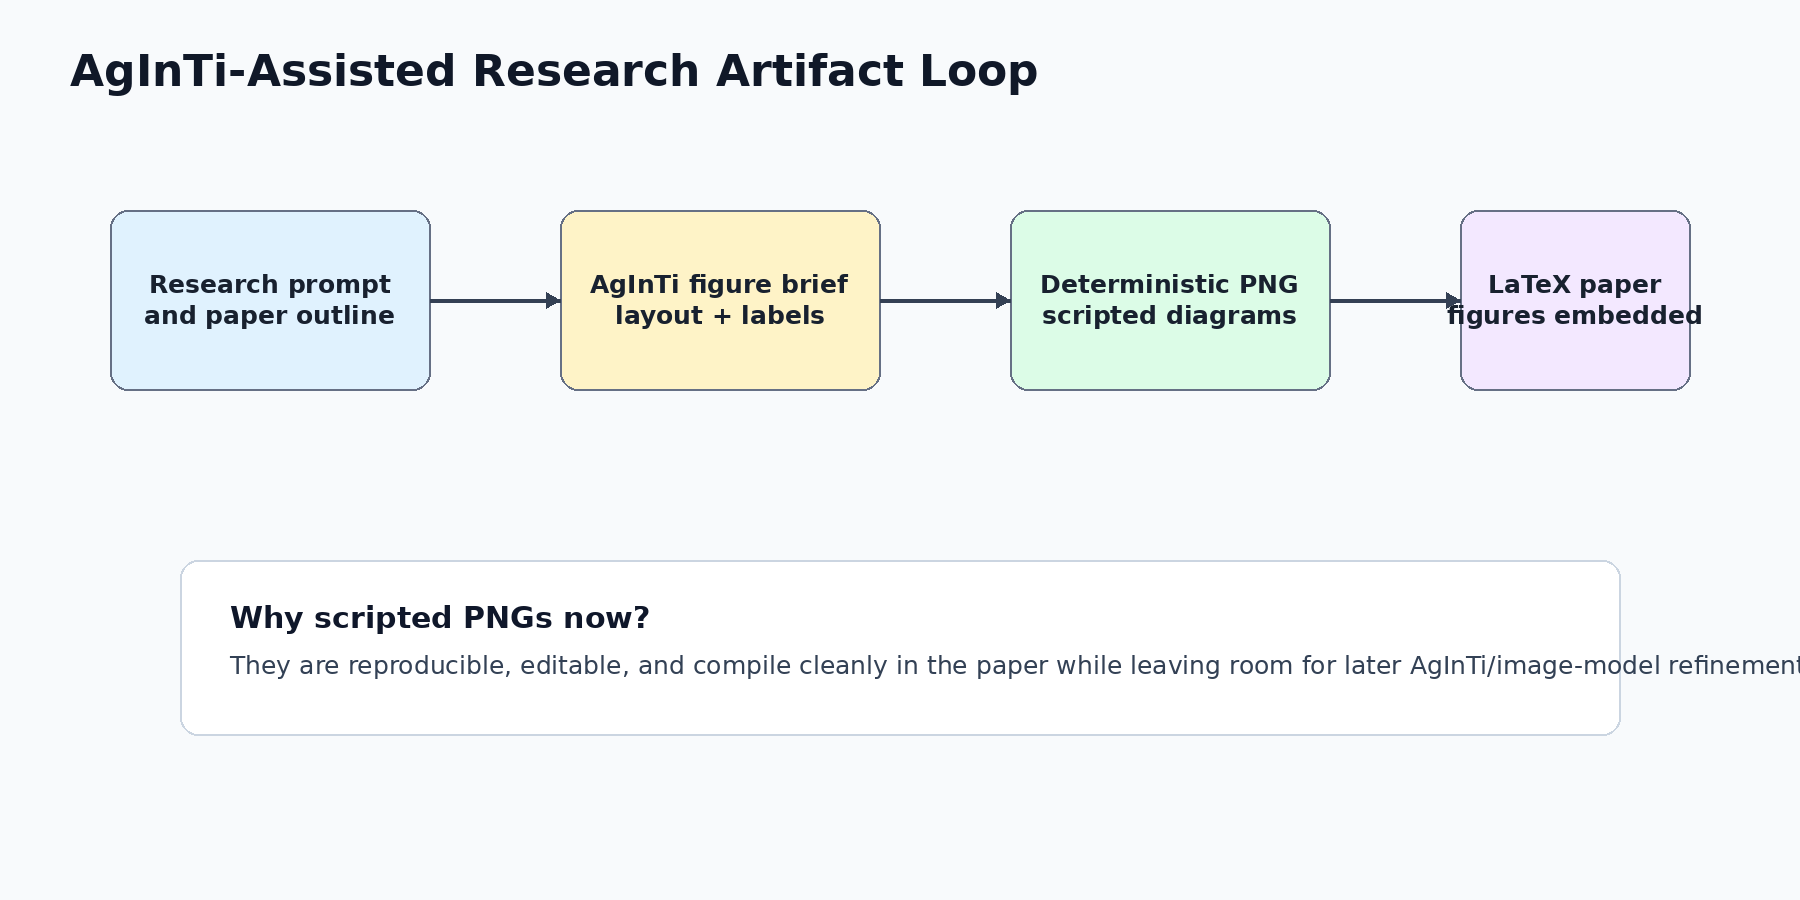
\includegraphics[width=\linewidth]{figures/aginti_artifact_loop.png}
  \caption{AgInTi-assisted artifact loop. The current figures are deterministic scripted PNGs so the paper is reproducible; the figure brief can later be sent to an interactive AgInTi/image agent for visual refinement.}
  \label{fig:aginti}
\end{figure}

The figure brief for AgInTi-style refinement is stored in the local AgInTi prompts subfolder. The current paper uses scripted PNG generation to keep the artifact reproducible.

\section{Evaluation}

The model should be evaluated as both a language model and a visual generator:
\begin{itemize}[leftmargin=*]
  \item Full-memory top-1/top-5 and reciprocal rank, not only within-batch accuracy.
  \item Separate results for same-wording rerenders and validated semantic paraphrases.
  \item OCR readability of genuinely generated modern text images, used only as an external metric.
  \item Human readability and task-success ratings.
  \item Glyph-stage retrieval accuracy: generated glyphs should retrieve correct characters and stages.
  \item Historical plausibility: distance to nearest real glyph exemplars in stage-specific embedding space.
  \item Layout validity: no text/panel overlap, stable reading order, correct answer composition.
  \item Image-to-image QA accuracy on rendered prompts and rendered answers.
\end{itemize}

\begin{center}
\begin{tabular}{p{0.26\linewidth}p{0.19\linewidth}p{0.42\linewidth}}
\toprule
System & Measured signal & Interpretation \\
\midrule
Whole-page flow & velocity MSE 0.851 & Unreadable page texture; negative baseline \\
Global visual memory & top-1 2.23\% over 2,016 & Above random, but 0/16 historical paraphrases \\
Causal InkStream & validation ink F1 0.639 & Autonomous repeated-grey collapse; negative baseline \\
Centered VFM & training in progress & Accept only after full-memory and paraphrase evaluation \\
\bottomrule
\end{tabular}
\end{center}

\section{Conclusion}

The experiments show that merely replacing tokens with pixels is insufficient. A page diffusion model can learn paper, and a causal pixel model can learn local strokes, without learning autonomous language. VFM instead treats visible language as an ordered semantic field coupled to amendable image-valued memory and protected historical evidence. The present code can establish image-only semantic reading and image answer recall on one GPU. It cannot yet claim unrestricted visual composition or parity with Qwen 8B. Those claims are reserved for the masked writer and a fixed benchmark, respectively.

\begin{thebibliography}{99}
\bibitem{gpt3} Brown et al. Language Models are Few-Shot Learners. \url{https://arxiv.org/abs/2005.14165}
\bibitem{gpt4} OpenAI. GPT-4 Technical Report. \url{https://arxiv.org/abs/2303.08774}
\bibitem{gpt4o} OpenAI. GPT-4o API model documentation. \url{https://developers.openai.com/api/docs/models/gpt-4o}
\bibitem{openaiimages} OpenAI. Images and Vision API documentation. \url{https://platform.openai.com/docs/guides/images-vision}
\bibitem{openaiimagegen} OpenAI. Image generation guide. \url{https://platform.openai.com/docs/guides/image-generation}
\bibitem{geminiimage} Google. Gemini API image generation documentation. \url{https://ai.google.dev/gemini-api/docs/image-generation}
\bibitem{llama3} Meta AI. The Llama 3 Herd of Models. \url{https://arxiv.org/abs/2407.21783}
\bibitem{donut} Kim et al. OCR-free Document Understanding Transformer. \url{https://arxiv.org/abs/2111.15664}
\bibitem{pix2struct} Lee et al. Pix2Struct: Screenshot Parsing as Pretraining for Visual Language Understanding. \url{https://arxiv.org/abs/2210.03347}
\bibitem{pixel} Rust et al. Language Modelling with Pixels. \url{https://arxiv.org/abs/2207.06991}
\bibitem{pixar} Tai et al. PIXAR: Auto-Regressive Language Modeling in Pixel Space. \url{https://arxiv.org/abs/2401.03321}
\bibitem{pixelgpt} Chai et al. Autoregressive Pre-Training on Pixels and Texts. \url{https://arxiv.org/abs/2404.10710}
\bibitem{canine} Clark et al. CANINE: Pre-training an Efficient Tokenization-Free Encoder. \url{https://arxiv.org/abs/2103.06874}
\bibitem{byt5} Xue et al. ByT5: Towards a Token-Free Future. \url{https://arxiv.org/abs/2105.13626}
\bibitem{megabyte} Yu et al. MEGABYTE: Predicting Million-byte Sequences with Multiscale Transformers. \url{https://arxiv.org/abs/2305.07185}
\bibitem{d3pm} Austin et al. Structured Denoising Diffusion Models in Discrete State-Spaces. \url{https://arxiv.org/abs/2107.03006}
\bibitem{diffusionlm} Li et al. Diffusion-LM Improves Controllable Text Generation. \url{https://arxiv.org/abs/2205.14217}
\bibitem{sedd} Lou et al. Discrete Diffusion Modeling by Estimating the Ratios of the Data Distribution. \url{https://arxiv.org/abs/2310.16834}
\bibitem{llada} Nie et al. Large Language Diffusion Models. \url{https://arxiv.org/abs/2502.09992}
\bibitem{maskgit} Chang et al. MaskGIT: Masked Generative Image Transformer. \url{https://arxiv.org/abs/2202.04200}
\bibitem{ldm} Rombach et al. High-Resolution Image Synthesis with Latent Diffusion Models. \url{https://arxiv.org/abs/2112.10752}
\bibitem{dit} Peebles and Xie. Scalable Diffusion Models with Transformers. \url{https://arxiv.org/abs/2212.09748}
\end{thebibliography}

\end{document}
